\documentclass{beamer}
\usepackage[utf8]{inputenc}
\usepackage{graphicx}
\author[Sowmya Vajjala]{Instructor: Sowmya Vajjala}


\title[LING 120]{LING 120, Fall 2017: \\ Language and Computers}
%\subtitle{based on Chapter 10 of the textbook}

\date{13 Sep 2017}

\institute{Iowa State University, USA}

%%%%%%%%%%%%%%%%%%%%%%%%%%%

\begin{document}

\begin{frame}\titlepage
\end{frame}

\begin{frame}
\frametitle{Class outline}%5minutes
\begin{enumerate}
\item Recap of last class
\item Issues involved in generating practice exercises automatically
\item Linguistic analysis necessary to create such exercises
\item An example learning support system, and an exercise in understanding its working
\end{enumerate}
\end{frame}

\begin{frame}
\frametitle{}
\begin{center}
\Large Quick recap of last class
\end{center}
\end{frame}

\begin{frame}
\frametitle{Computer Assisted Language Learning}
Advantages: 
\begin{itemize}
\item Individualized, personal feedback
\item More and more practice with specific patterns of language, idioms of the language etc. 
\item No worries about limited classroom interaction with the instructor
\item Unlike humans, a computer is objective with all students
\end{itemize} \pause
Questionable stuff: 
\begin{itemize}
\item Can we trust a computer?
\item Is it really possible to build such systems?  
\item Is it really free of bias?
\end {itemize}
\end{frame}


\begin{frame}
\frametitle{Some tasks an intelligent CALL system should do}
\begin{itemize}
\item Generate different kinds of questions
\item Automatically evaluate answers
\item Show different kinds of reading materials (from the web too, if needed - not limited to selected frames)
\item Give feedback to learners if they make mistakes.
\end{itemize}
... 
\end{frame}

\begin{frame}
\frametitle{Yesterday's exercise}
\begin{itemize}
\item Let us take this passage \small{\textit{The company was founded in 2009 by Alex Shevchenko and Max Lytvyn. Brad Hoover, the company's chief executive officer, is an investor with a background in engineering who learned about Grammarly while searching for an automated proofreading tool for his own writing. Grammarly, Inc, has headquarters in San Francisco. An additional office is in Kiev.}}
\normalsize \item If I asked you to create multiple choice questions from this, what questions will you create? and why? 
\item Write down your questions on a paper and the choices, and the rationale behind choosing them.
\item Work in groups of 2--3 people. Write your names on the paper and return it to me. This counts as your attendance for today. 
\end{itemize}
\end{frame}

\begin{frame}
\frametitle{Comments on Your answers}
\begin{itemize}
\item There are several person names, so there can be a question related to names and writing combinations of names can create confusion while answering.
\item There are several place names, so question can be asked about that.
\item Question about year.
\item Questions testing grammar (capitalization, missing apostrophe etc)
\end{itemize}
\end{frame}

\begin{frame}
\frametitle{}
\begin{center}
\Large How can a computer create tutor and test automatically?
\end{center}
\end{frame}

\begin{frame}
\frametitle{What kind of things should a computer know?}
\framesubtitle{Reading and Writing}
\begin{itemize}
\item break up sentences into individual words (called tokenization)
\item Identify different parts-of-speech (to generate say questions that test prepositions), different forms a word etc
\item Identify names of people, organizations, places, years etc (to generate factual, one word answer questions)
\item Identify synonyms of a word, other related words such as hypernyms (Color is the hypernym of Red. Red is the hyponym of Color) etc. (Why?) 
\end{itemize} \pause
.. okay, may be all the others are difficult tasks. But, breaking up into words??
\end{frame}

\begin{frame}
\frametitle{is tokenization even a problem?}
\begin{itemize}
\item In the sentence: "Umm, I don't know .... it is perhaps a good idea to talk to a Dr. Vajjala instead of a laptop computer!", how many words are there? \pause
\item Is Umm  a word?
\item Is "don't" one word or two?
\item Does the dot after Dr mean a break into new sentence? or just a title?
\item Should "laptop computer" be considered as one "compound" word? or two separate, unrelated words?
\item Should we separate out those punctuations or keep them with words?
\end{itemize}
... a computer needs to concern itself about these issues. 
\end{frame}

\begin{frame}
\frametitle{What kind of things should a computer know?}
\framesubtitle{Speaking and Listening}
\begin{itemize}
\item break up speech into individual words 
\item Check for your pronunciation
\item Other tasks can remain same here too.
\end{itemize}
\end{frame}

\begin{frame}
\frametitle{How will it give back some feedback?}
\begin{itemize}
\item It should understand what is missing in your answers.
\item Let us say you used a wrong tense (i.e., it should know how to do grammar check)
\item It should be able to generated a feedback sentence by itself and show/speak that to you. 
\\ ("You missed a tense" can be a canned response. "In this sentence, you made a mistake with the tense of the verb pass" is a "generated" sentence)
\end{itemize}
\end{frame}

\begin{frame}
\frametitle{Modeling the learner}
\begin{itemize}
\item  Keeping track of progress
\item Understanding what a learner is doing well, what are her weak points
\item over-use or under-use of specific language structures
\item How to give personalized feedback (e.g., specific to the learner's native language background)
\item sequencing of teaching materials
\item prioritizing feedback (if there are several errors, should the system just keep putting red-marks all over, or prioritize one feedback over another?)
\item plagiarism detection
\end{itemize}
.... and so on
\end{frame}

\begin{frame}
\frametitle{An Example CALL system}
\begin{itemize}
\item TAGARELA: Teaching Aid for Grammatical Awareness, Recognition and Enhancement of Linguistic Abilities
\item a web-based workbook for teaching specific aspects of grammar.
\item Website: \url{http://sifnos.sfs.uni-tuebingen.de/tagarela/index.py/main}
\item Some aspects of TAGARELA (from a 2010 talk): \url{http://www.sfs.uni-tuebingen.de/~dm/handouts/barcelona-10-10-26.pdf}
\end{itemize}
\end{frame}

\begin{frame}
\frametitle{Other examples of tutoring/learning support systems}
Next class!
\end{frame}

\begin{frame} %15min?
\frametitle{Attendance exercise} \framesubtitle{post answers on Canvas forum for today}
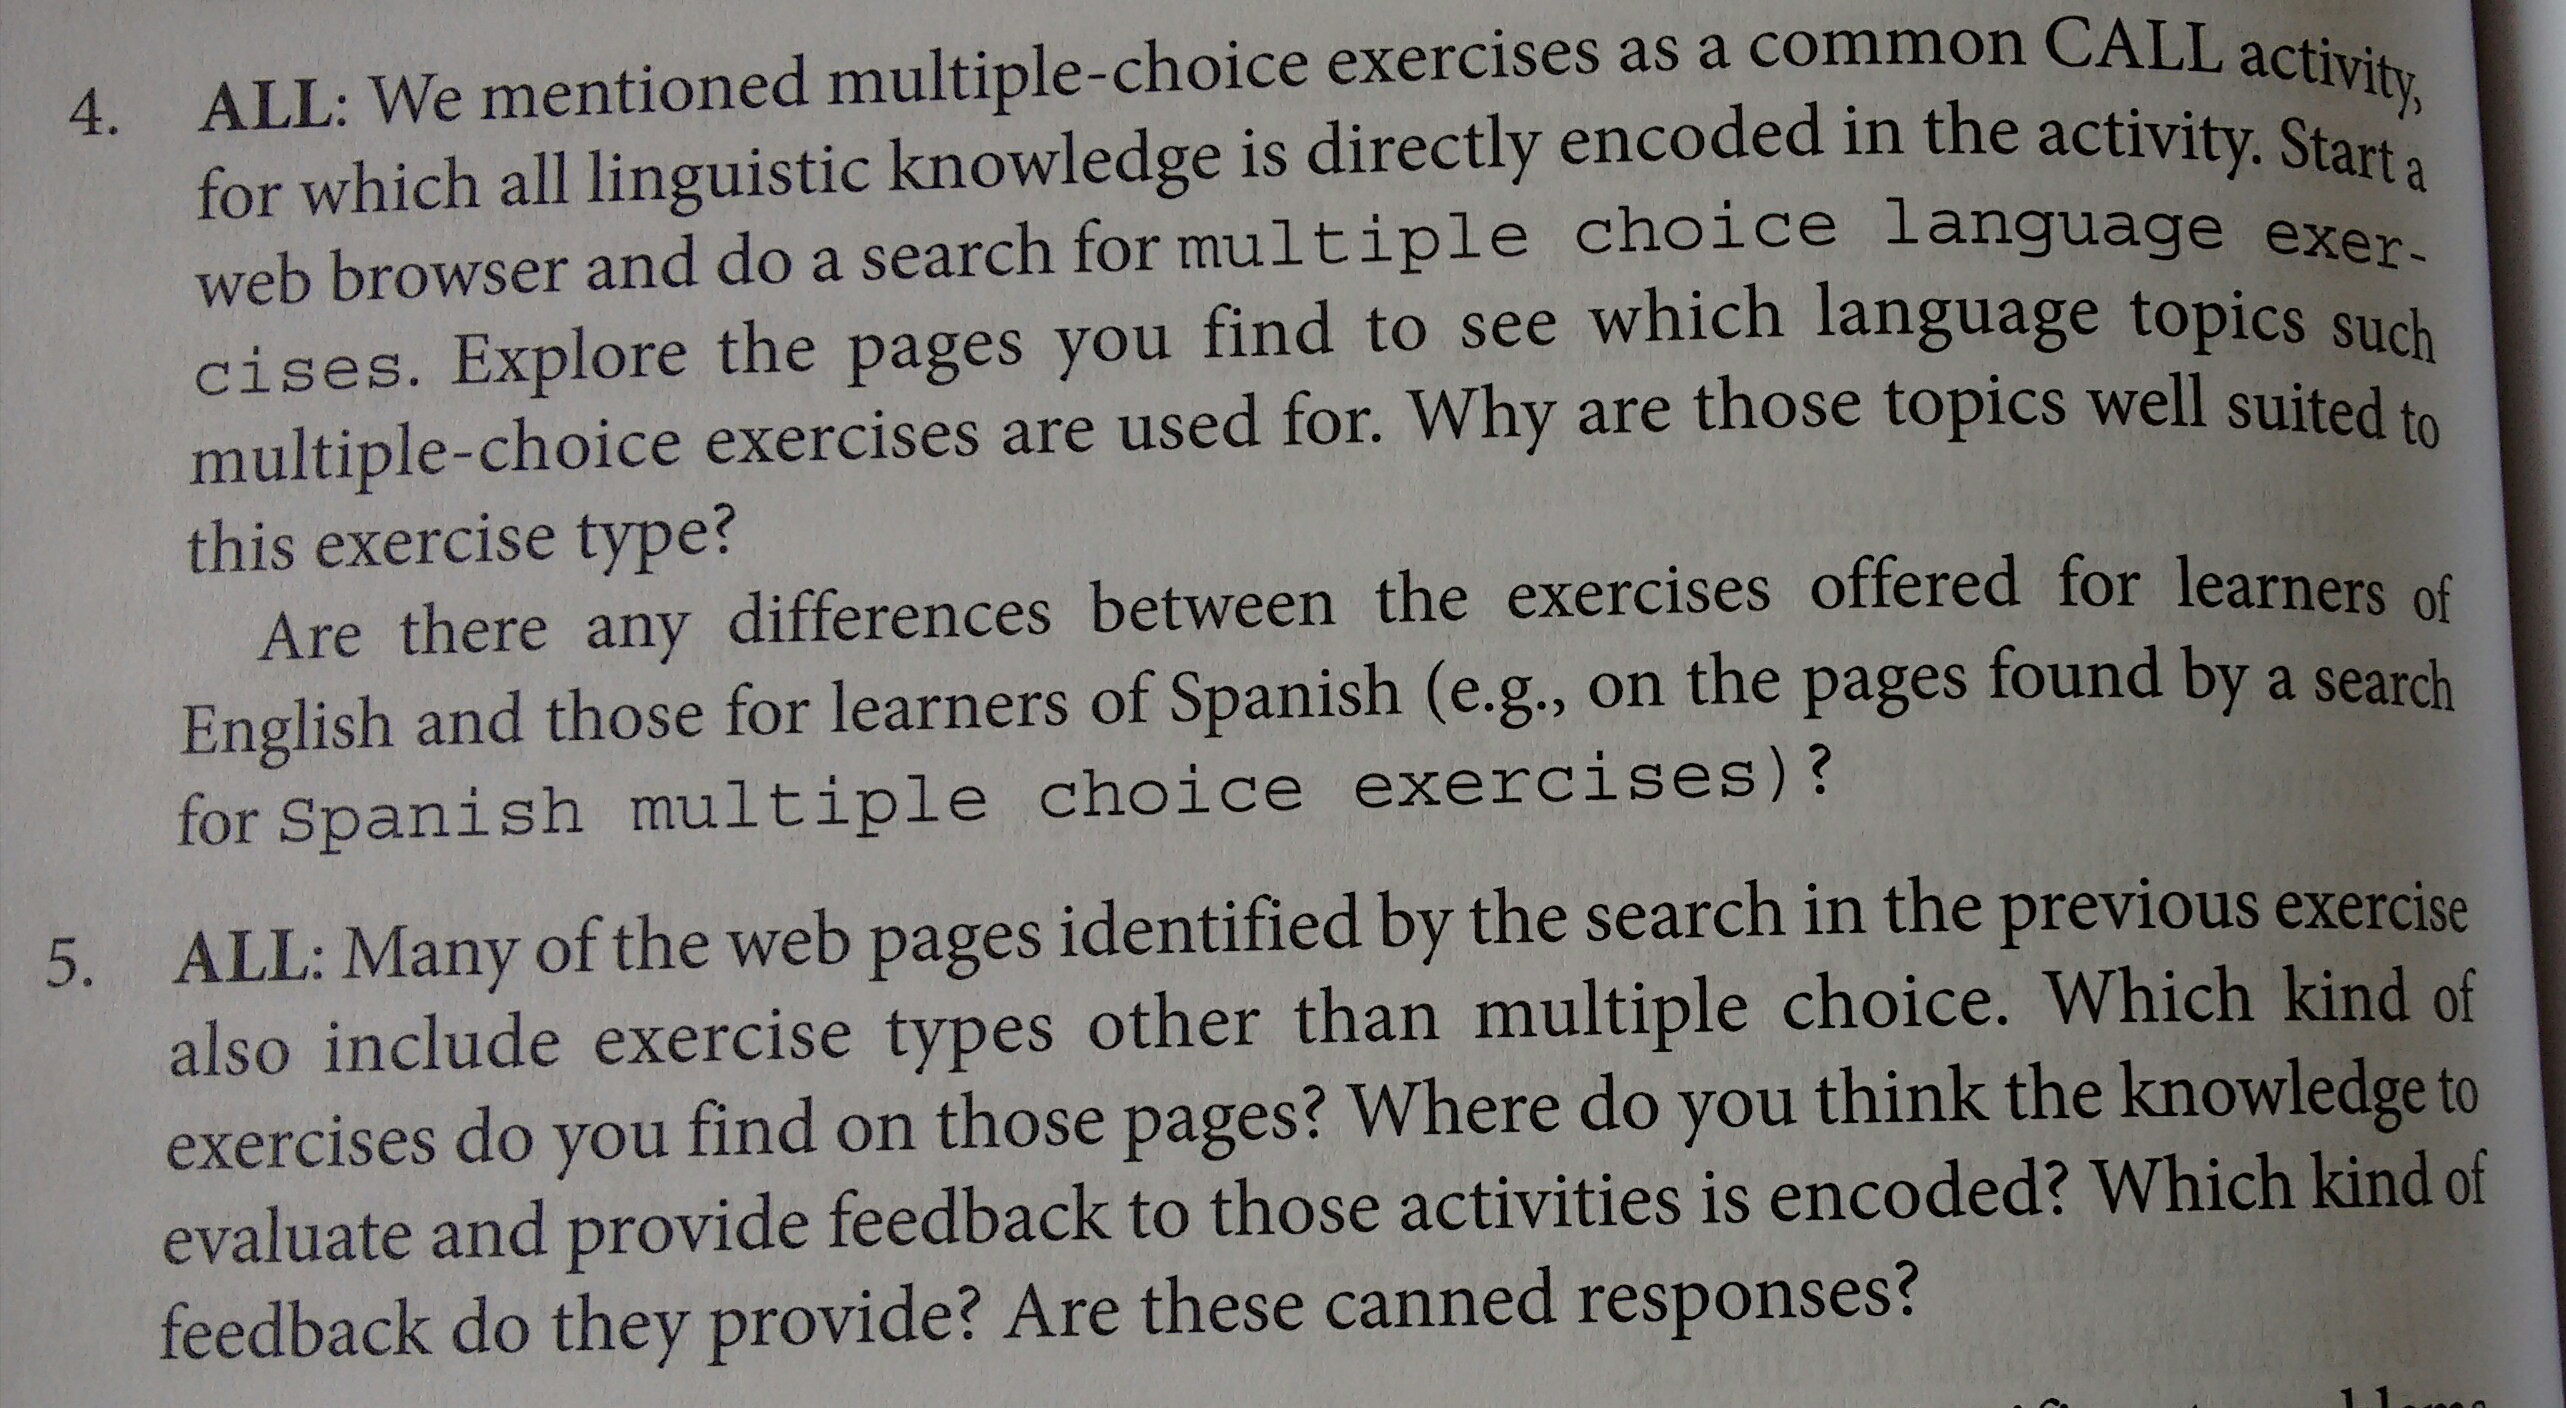
\includegraphics[width=0.99\textwidth]{13SepExercise.jpg}
\end{frame}

\end{document}
